\section{Systematic Uncertainties and Result}
\label{sec:syst}
\emph{In short: thirteen variants in four groups give a systematic uncertainty of $0.0070$ (Bayesian) and $0.0072$ (frequentist), dominated by the particle-identification requirement; the final result is $\Araw=-0.0443\pm0.0085\,(\text{stat})\pm0.0070\,(\text{syst})$.}
The systematic study asks how much the result depends on choices of the analysis that the data do not fix. The frequentist and Bayesian fits share one study, so that the two uncertainties are comparable: the same thirteen variants of the nominal choices, fitted by both methods on exactly the same candidates, and the same rule to combine them. The variants (listed in Table~\ref{tab:syst}) change one choice at a time and fall in four groups: the \emph{window}, the \emph{background} model, the \emph{signal} model and the \emph{preselection} cuts.

The shift $\Delta=\Araw^{\mathrm{var}}-\Araw^{\mathrm{nom}}$ of a variant is not necessarily a systematic effect: when a variant changes the sample (window, preselection) the two samples are nested and part of $\Delta$ is a statistical fluctuation of expected size $\sigma_B=\sqrt{|\sigma_{\mathrm{var}}^2-\sigma_{\mathrm{nom}}^2|}$~\cite{barlow}, and such a variant contributes only if $|\Delta|>\sigma_B$. A variant that the data reject ($\Delta\chi^2>25$ on the same data) is excluded: this removes the single exponential ($\Delta\chi^2=134$, Appendix~\ref{sec:bayes_gof}). The largest remaining $|\Delta|$ of each group is its uncertainty, since the variants of a group are alternative descriptions of the same choice, and the groups, being independent choices, are added in quadrature.

\begin{table*}[t]
\centering
\resizebox{\ifdim\width>\linewidth\linewidth\else\width\fi}{!}{\begin{tabular}{llrrrrr}
\toprule
Group & Variant & $n$ & $\Delta$ Bayes & $\sigma_B$ Bayes & $\Delta$ freq. & $\sigma_B$ freq. \\
\midrule
Window & $[5050,5600]$ & $21164$ & $-0.0003$ & $0.0009$ & $-0.0004$ & $0.0005$ \\
 & $[5150,5600]$ & $18566$ & $-0.0001$ & $0.0007$ & $-0.0005$ & $0.0021$ \\
 & $[5100,5450]$ & $19004$ & $+0.0002$ & $0.0009$ & $-0.0001$ & $0.0003$ \\
 & $[5100,5700]$ & $20191$ & $\mathbf{-0.0014}$ & $0.0010$ & $\mathbf{-0.0014}$ & $0.0001$ \\
Background & single exponential (rejected) & $19731$ & $-0.0037$ & -- & $-0.0039$ & -- \\
 & shape shared between charges & $19731$ & $\mathbf{-0.0037}$ & -- & $\mathbf{-0.0040}$ & -- \\
 & symmetric, $A_b=0$ & $19731$ & $-0.0028$ & -- & $-0.0031$ & -- \\
Signal & Crystal Ball & $19731$ & $\mathbf{-0.0002}$ & -- & $\mathbf{-0.0006}$ & -- \\
 & $\mu,\sigma$ per charge & $19731$ & $-0.0000$ & -- & $-0.0001$ & -- \\
Preselection & $\texttt{ProbK}>0.4$ & $26553$ & $-0.0032$ & $0.0038$ & $-0.0032$ & $0.0037$ \\
 & $\texttt{ProbK}>0.6$ & $13981$ & $\mathbf{+0.0058}$ & $0.0048$ & $\mathbf{+0.0058}$ & $0.0050$ \\
 & $\texttt{ProbPi}<0.4$ & $17984$ & $+0.0022$ & $0.0022$ & $+0.0020$ & $0.0023$ \\
 & $\texttt{ProbPi}<0.6$ & $20953$ & $-0.0004$ & $0.0020$ & $-0.0006$ & $0.0017$ \\
\midrule
\multicolumn{3}{l}{Group uncertainties: window / background / signal / preselection} & \multicolumn{2}{c}{$0.0014/0.0037/0.0002/0.0058$} & \multicolumn{2}{c}{$0.0014/0.0040/0.0006/0.0058$} \\
\multicolumn{3}{l}{Total (quadrature)} & \multicolumn{2}{c}{$0.0070$} & \multicolumn{2}{c}{$0.0072$} \\
\bottomrule
\end{tabular}}
\caption{Systematic study common to the Bayesian and frequentist fits: shift of $\Araw$ for each variant and, for the variants that change the sample, the expected statistical spread $\sigma_B$ of the shift. The largest contributing shift of each group is in bold. The single exponential is rejected by the data and excluded. For the window $[5150,5600]$ the frequentist uncertainty is scaled from the number of events, since the Hesse matrix of that fit is not accurate.}
\label{tab:syst}
\end{table*}

The results are in Table~\ref{tab:syst}, and all the Bayesian fits in Table~\ref{tab:bayes_all} of Appendix~\ref{sec:syst_tables}. The two methods give the same shifts to within $\sim$$0.0005$ and the same group uncertainties, with totals of $0.0070$ (Bayesian) and $0.0072$ (frequentist):
\begin{gather*}
\text{Bayesian:}\\ \Araw=-0.0443\pm0.0085\,(\text{stat})\pm0.0070\,(\text{syst}),\\[2pt]
\text{frequentist:}\\ \Araw=-0.0441\pm0.0085\,(\text{stat})\pm0.0072\,(\text{syst}).
\end{gather*}

The preselection dominates, through the single variant $\texttt{ProbK}>0.6$ ($+0.0058$, $1.2\,\sigma_B$). The scan of each cut in steps of $0.05$ (Fig.~\ref{fig:syst_pid_scan} of Appendix~\ref{app:syst}) shows that this value is a fluctuation: on the tight side the shifts scatter around zero within $1.3\,\sigma_B$ without a trend, whereas loosening $\texttt{ProbK}$ moves $\Araw$ monotonically, as expected if misidentified decays not in the mass model enter the sample. The nominal requirement is therefore well placed and the preselection uncertainty conservative. The background group is second, driven by the charge dependence of the background, and the window third.

\subsection{Stability Checks of the Frequentist Fit}
\label{sec:freq_syst}
While the systematic uncertainties study is shared with the Bayesian approach -- and discussed in detail in Sec.~\ref{sec:syst} -- three specific stability checks were performed within the frequentist one, to evaluate the robustness of the fitted raw asymmetry $\Araw$. Each test consists of a two-dimensional grid scan in which two selection or fit parameters are varied simultaneously, performing a simultaneous fit with the nominal double-exponential background model at each point and observing the stability of $\Araw$.

\begin{enumerate}[leftmargin=*]
    \item \textbf{Fit Window Scan:} The lower and upper boundaries of the invariant mass fit window, nominally set to $[5100, 5600]\,\MeV$, were scanned over the ranges $[5000, 5200]\,\MeV$ and $[5350, 6100]\,\MeV$, respectively, with a 50 \MeV step. This test evaluates the sensitivity of $\Araw$ to the exponential background parametrization, and is useful to choose the nominal window: too small or too asymmetric fit window produces unstable fit, due to worse background estimation.

    \item \textbf{Signal Region Scan:} Changing the extremes of the signal region not significant fluctation in $\Araw$ are observed, suggesting that the sideband preliminar fit could be avoided.

    \item \textbf{Particle Identification Cut Scan:} The preselection cuts on the final-state kaon PID likelihoods (\texttt{ProbK} and \texttt{ProbPi}) were varied simultaneously towards a better kaon purity (larger than $0.5$ for kaons, smaller than $0.5$ for pions). This influences significantly the $\Araw$ estimation, but always within the $68\%$ CI, confirming the cut selection as reasonable.
\end{enumerate}

The three grids are shown in Fig.~\ref{fig:freq_stability}.

\begin{figure*}[t]
\centering
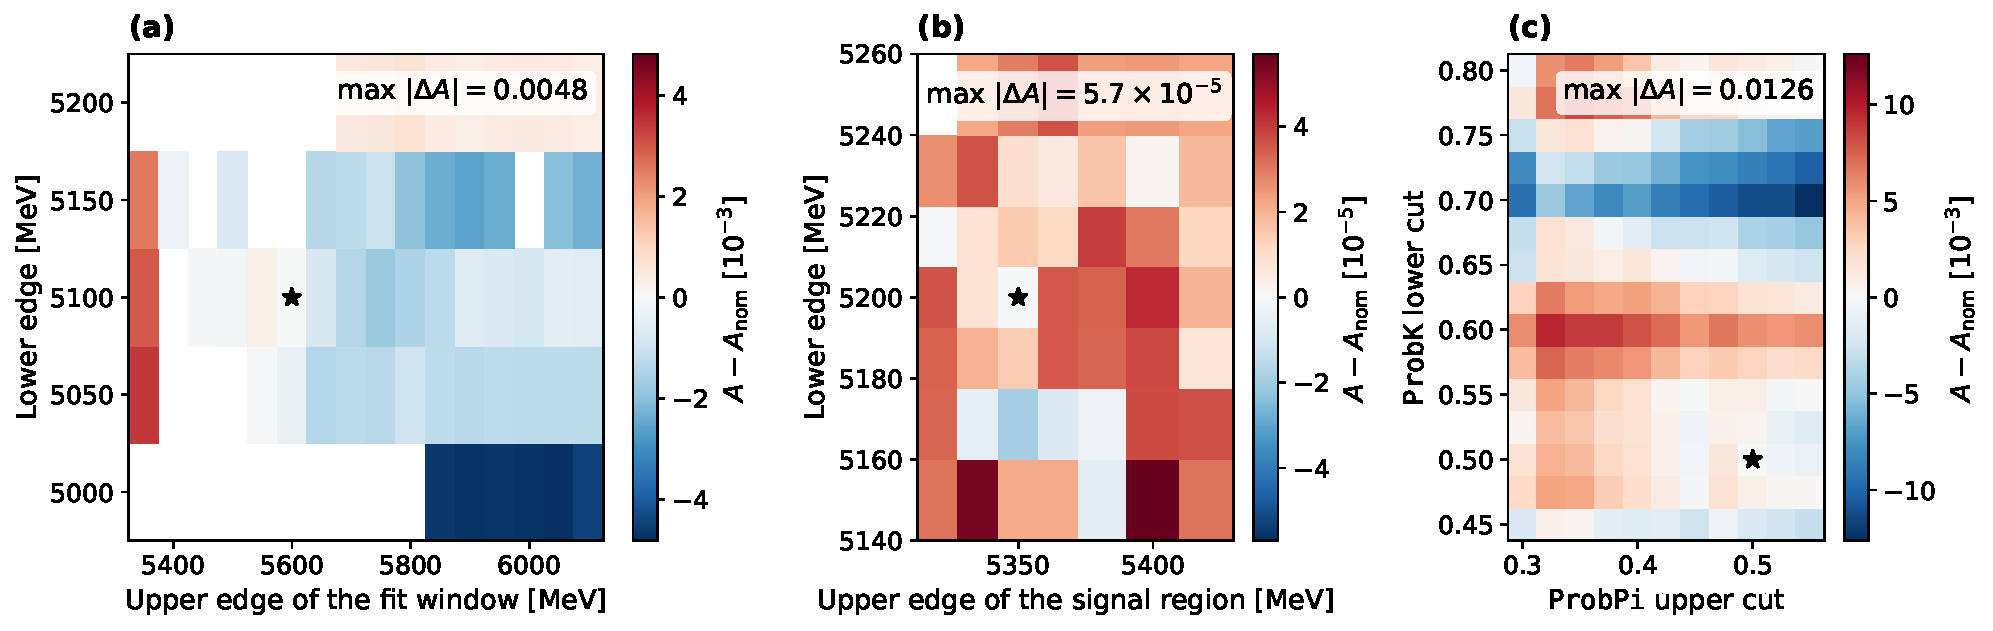
\includegraphics[width=0.95\textwidth]{figures/freq_stability.pdf}
\caption{Stability of the fitted $\Araw$ over the three grids: (a) lower and upper edge of the fit window (only fits with a valid minimum and an accurate covariance are shown); (b) lower and upper edge of the signal region; (c) lower cut on \texttt{ProbK} and upper cut on \texttt{ProbPi}. The colour is the shift with respect to the nominal fit (star), in units of $10^{-3}$ for (a) and (c) and $10^{-5}$ for (b); the statistical uncertainty of the nominal fit is $8.5\times10^{-3}$.}
\label{fig:freq_stability}
\end{figure*}

Across all scan configurations, the maximum observed variation in $\Araw$ remains below the statistical uncertainty ($\Delta \Araw < \sigma_{\mathrm{stat}}$), demonstrating the stability of the nominal fit result.

The numbers of the three scans are given in Appendix~\ref{sec:freq_stab_numbers}.
